\documentclass{article}
%\documentclass[draft]{article}     % use draft option in packages
%=============================
% preamble
%=============================
\usepackage[utf8]{inputenc}         % use UTF-8 encoding
\usepackage{graphicx}               % insert images
%\usepackage[draft]{graphicx}        % do not render figures
\usepackage[english]{babel}         % use English language

\graphicspath{                      % path for figures
    {../figures/} 
    {../figures/memes} 
}

%-----------------------------
\title{NSGC - Neural Spell \& Grammar Checker (en/pt)}
\author{Rafael Ito}
\date{June 2020}

%=============================
% body
%=============================
\begin{document}

\maketitle

\begin{abstract}
%------------------------

https://github.com/dl4nlp-rg/PF06-RIto
%------------------------
\end{abstract}

%=================================================
\section{Introduction}
%=================================================

This is an example of paper citation: BERT~\cite{devlin2018bert} is a transformer. T5~\cite{raffel2019exploring} also uses transformers.

%=================================================
\section{Methodology} 
%=================================================

This is an example of inserting a figure. 

\begin{figure}[ht]
\centering
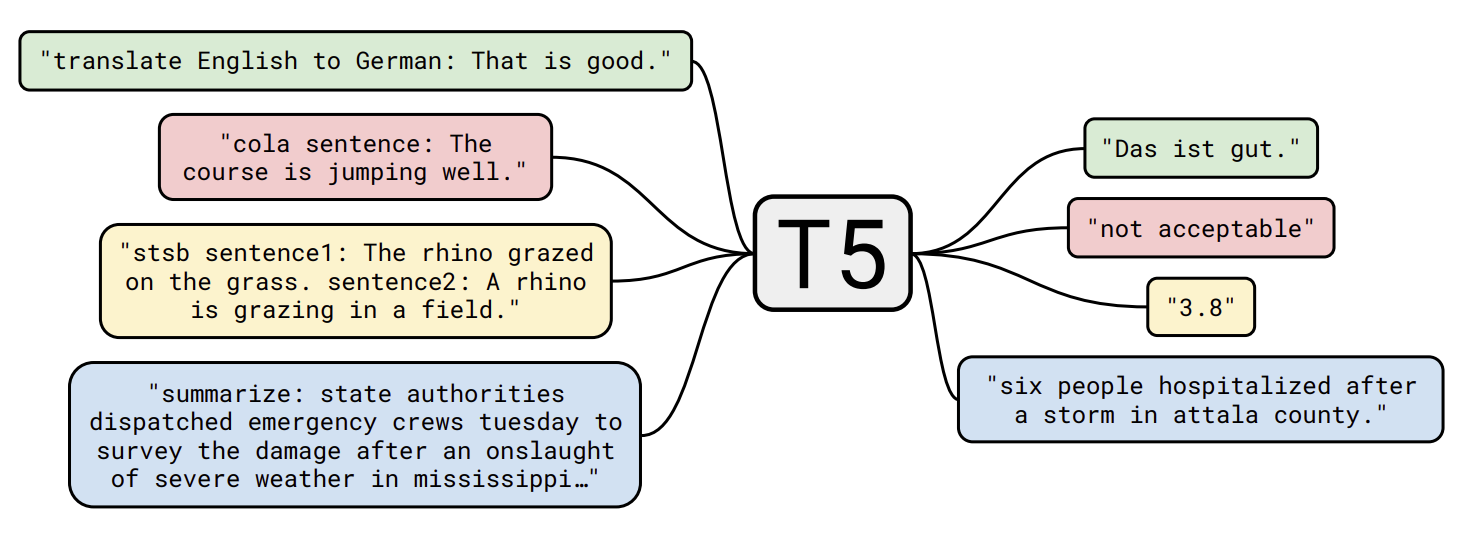
\includegraphics[width=.77\textwidth]{t5.png}
\caption{\label{fig:t5}Figure example.}
\end{figure}

Figure~\ref{fig:t5} is an example of figure citation.

%------------------------
\subsection{Metrics}
%------------------------

%------------
\subsubsection{$M^2$ (MaxMatch)}
%------------

%------------
\subsubsection{GLEU}
%------------

%------------
\subsubsection{Edit distance}
%------------

%=================================================
\section{Data set}
%=================================================

%------------------------
\subsection{CoNLL-2013}
%------------------------

%------------------------
\subsection{CoNLL-2014}
%------------------------

%------------------------
\subsection{JFLEG}
%------------------------

%------------------------
\subsection{BEA}
%------------------------

%------------------------
\subsection{ReGRA}
%------------------------


%=================================================
\section{Experiments}
%=================================================

%=================================================
\section{Conclusion}
%=================================================

%=================================================
\section{Future Work}
%=================================================

%-------------------------------------------------
\subsection{}
%-------------------------------------------------
%=================================================
% Bibliography
%=================================================

%------------------------
%% Architectures
%BERT~\cite{devlin2018bert}
%T5~\cite{raffel2019exploring}
%Transformer~\cite{vaswani2017attention}
%%------------------------
%% GEC shared tasks
%HOO~\cite{dale2010helping}
%HOO-2011~\cite{dale2011helping}
%HOO-2012~\cite{dale2012hoo}
%CoNLL-2013~\cite{ng-etal-2013-conll}
%CoNLL-2014~\cite{ng2014conll}
%JFLEG~\cite{napoles2017jfleg}
%BEA~\cite{bryant2019bea}
%%------------------------
%% GEC Systems
%Encoder-Decoder~\cite{kaneko2020encoder}
%Soft-Masked BERT~\cite{zhang2020spelling}
%GECToR~\cite{omelianchuk2020gector}
%ReGRA~\cite{nunes2000processo}
%%------------------------
%% Datasets
%CoNLL-2013~\cite{ng-etal-2013-conll}
%CoNLL-2014~\cite{ng2014conll}
%JFLEG~\cite{napoles2017jfleg}
%BEA~\cite{bryant2019bea}
%ReGRA~\cite{nunes2000processo}
%%------------------------
%% Corpus
%Write \& Improve~\cite{yannakoudakis2018developing}
%LOCNESS~\cite{granger1998computer}
%%------------------------
%% Metrics
%GLEU~\cite{napoles2015ground}
%GLEU improved~\cite{napoles2016gleu}
%ERRANT~\cite{bryant-etal-2017-automatic}
%MaxMatch~\cite{dahlmeier2012better}
%%------------------------

% Usando a bibliografia com arquivo no formato bibtex, (ver arquivo main.bib que faz parte desse projeto)
\bibliographystyle{plain}
\bibliography{main.bib}

\end{document}
